\documentclass[aspectratio=169]{beamer}

\usetheme{Madrid}
\usecolortheme{seahorse}
\usefonttheme{professionalfonts}

\usepackage{listings}
\usepackage{xcolor}
\usepackage{tikz}
\usepackage{booktabs}
\usepackage{hyperref}
\usepackage{textcomp}
\usepackage{microtype}

\definecolor{codebg}{HTML}{1E1E2E}
\definecolor{codegreen}{HTML}{A6E3A1}
\definecolor{codeblue}{HTML}{89DCEB}
\definecolor{codeyellow}{HTML}{F9E2AF}
\definecolor{codegray}{HTML}{6C7086}
\definecolor{codepurple}{HTML}{CBA6F7}
\definecolor{codeorange}{HTML}{FAB387}
\definecolor{codewhite}{HTML}{CDD6F4}
\definecolor{alertred}{HTML}{F38BA8}

\lstdefinestyle{clang}{
  backgroundcolor=\color{codebg},
  basicstyle=\ttfamily\footnotesize\color{codewhite},
  keywordstyle=\color{codepurple}\bfseries,
  commentstyle=\color{codegray}\itshape,
  stringstyle=\color{codegreen},
  numberstyle=\tiny\color{codegray},
  numbers=left, numbersep=6pt,
  breaklines=true, frame=single,
  rulecolor=\color{codeblue},
  language=C,
  tabsize=4
}

\lstdefinestyle{asm}{
  backgroundcolor=\color{codebg},
  basicstyle=\ttfamily\footnotesize\color{codewhite},
  keywordstyle=\color{codepurple}\bfseries,
  commentstyle=\color{codegray}\itshape,
  stringstyle=\color{codegreen},
  numberstyle=\tiny\color{codegray},
  numbers=left, numbersep=6pt,
  breaklines=true, frame=single,
  rulecolor=\color{codepurple},
  tabsize=4
}

\title[MyOS Chapter 4]{\textbf{MyOS Chapter 4: Permanent Interrupt Architecture}}
\subtitle{From temporary guards to full ISR/IRQ framework}
\author{MyOS Project}
\date{March 2026}
\institute{x86 Protected Mode Kernel Engineering}

\newcommand{\concept}[2]{%
  \begin{block}{#1}\smallskip #2\smallskip\end{block}\vspace{5pt}}

\newcommand{\warn}[1]{%
  \begin{alertblock}{Important}\smallskip #1\smallskip\end{alertblock}\vspace{5pt}}

\begin{document}

\begin{frame}
  \titlepage
\end{frame}

\begin{frame}{Why the temporary fix was not enough}
  \begin{itemize}
    \item Masking IRQ lines reduces crashes but does not define real exception/IRQ flow
    \item Missing structured stubs can corrupt stack on different vectors
    \item No central dispatcher means duplicated or inconsistent interrupt logic
  \end{itemize}
  \vspace{6pt}
  \concept{Permanent goal}{
    Build a full path for vectors 0--47 with shared ABI, C-level dispatch, and deterministic PIC EOI behavior.
  }
\end{frame}

\begin{frame}{Final Architecture}
  \begin{center}
  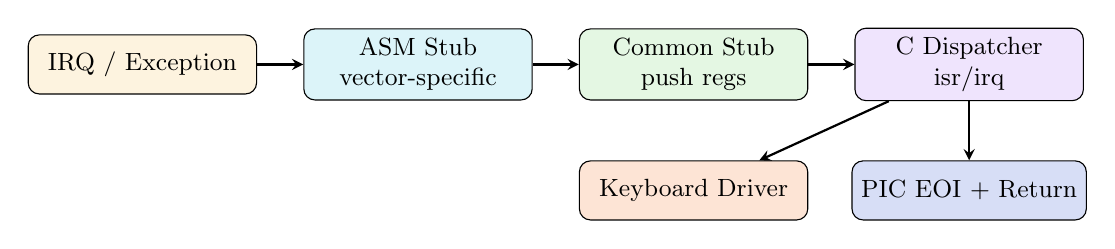
\begin{tikzpicture}[
      box/.style={rectangle,draw,rounded corners=4pt,
                  minimum width=2.9cm,minimum height=0.75cm,
                  align=center,font=\small},
      arr/.style={->,thick,>=stealth}]
    \node[box,fill=codeyellow!40] (irq) at (0,0) {IRQ / Exception};
    \node[box,fill=codeblue!30]   (stub) at (3.5,0) {ASM Stub\\vector-specific};
    \node[box,fill=codegreen!30]  (common) at (7.0,0) {Common Stub\\push regs};
    \node[box,fill=codepurple!30] (cdisp) at (10.5,0) {C Dispatcher\\isr/irq};

    \node[box,fill=codeorange!35] (kbd) at (7.0,-1.6) {Keyboard Driver};
    \node[box,fill=codewhite!80]  (eoi) at (10.5,-1.6) {PIC EOI + Return};

    \draw[arr] (irq) -- (stub);
    \draw[arr] (stub) -- (common);
    \draw[arr] (common) -- (cdisp);
    \draw[arr] (cdisp) -- (kbd);
    \draw[arr] (cdisp) -- (eoi);
  \end{tikzpicture}
  \end{center}
\end{frame}

\begin{frame}[fragile]{Assembly Stub Generation Strategy}
  \begin{lstlisting}[style=asm]
%macro ISR_NOERR 2
%1:
    push dword 0
    push dword %2
    jmp isr_common_stub
%endmacro

%macro ISR_ERR 2
%1:
    push dword %2
    jmp isr_common_stub
%endmacro

%macro IRQ_STUB 2
%1:
    push dword 0
    push dword %2
    jmp irq_common_stub
%endmacro
  \end{lstlisting}
  \textbf{Line logic:}
  \begin{itemize}
    \item Exceptions without CPU error code get synthetic \texttt{err\_code=0}
    \item Exceptions with CPU error code preserve it and only push vector number
    \item IRQ vectors always push synthetic error code + vector number
  \end{itemize}
\end{frame}

\begin{frame}[fragile]{Common Stub ABI (ASM \textrightarrow C)}
  \begin{lstlisting}[style=asm]
isr_common_stub:
    pusha
    cld
    push esp
    call isr_handler
    add esp, 4
    popa
    add esp, 8
    iretd

irq_common_stub:
    pusha
    cld
    push esp
    call irq_handler
    add esp, 4
    popa
    add esp, 8
    iretd
  \end{lstlisting}
  \concept{Why this is stable}{
    Every vector follows one stack contract. C receives a single \texttt{registers\_t*} view of CPU state.
  }
\end{frame}

\begin{frame}[fragile]{C Dispatcher Structures}
  \begin{lstlisting}[style=clang]
typedef struct {
    uint32_t edi, esi, ebp, esp;
    uint32_t ebx, edx, ecx, eax;
    uint32_t int_no, err_code;
    uint32_t eip, cs, eflags;
} registers_t;
  \end{lstlisting}
  \textbf{Logic behind order:}
  \begin{itemize}
    \item Matches \texttt{pusha} register push order exactly
    \item Then matches the stub-pushed metadata: \texttt{int\_no}, \texttt{err\_code}
    \item Then CPU-saved return frame: \texttt{eip/cs/eflags}
  \end{itemize}
\end{frame}

\begin{frame}[fragile]{Exception Path: \texttt{isr\_handler()}}
  \begin{lstlisting}[style=clang]
void isr_handler(registers_t* regs) {
    set_color(0x0C);
    print("\n\n[EXCEPTION] ");
    print(exception_messages[regs->int_no]);
    print(" (#");
    print_int((int)regs->int_no);
    print(") err=");
    print_int((int)regs->err_code);
    print("\nSystem halted.\n");
    cli; hlt-loop;
}
  \end{lstlisting}
  \warn{Critical design choice: halt on exception instead of silent reboot. This makes faults debuggable.}
\end{frame}

\begin{frame}[fragile]{IRQ Path: \texttt{irq\_handler()}}
  \begin{lstlisting}[style=clang]
void irq_handler(registers_t* regs) {
    if (regs->int_no == 33) {
        keyboard_irq_handler();
    }

    if (regs->int_no >= 40) {
        outb(0xA0, 0x20);
    }
    outb(0x20, 0x20);
}
  \end{lstlisting}
  \textbf{Line logic:}
  \begin{itemize}
    \item Dispatches IRQ1 to keyboard only
    \item Sends EOI to slave PIC for IRQ8--15 first
    \item Always sends EOI to master PIC
  \end{itemize}
\end{frame}

\begin{frame}[fragile]{IDT Wiring: Full 0--47 Coverage}
  \begin{lstlisting}[style=clang]
idt_set_gate(0,  (uint32_t)isr0);
...
idt_set_gate(31, (uint32_t)isr31);

idt_set_gate(32, (uint32_t)irq0);
...
idt_set_gate(47, (uint32_t)irq15);
  \end{lstlisting}
  \concept{Permanent improvement}{
    No empty vectors in the active interrupt space. Unexpected IRQ/exception now has deterministic behavior.
  }
\end{frame}

\begin{frame}[fragile]{PIC Remap Reliability}
  \begin{lstlisting}[style=clang]
outb(0x20, 0x11); io_wait();
outb(0xA0, 0x11); io_wait();
...
outb(0x21, 0xFD); io_wait();  // only IRQ1 unmasked
outb(0xA1, 0xFF); io_wait();  // all slave IRQs masked
  \end{lstlisting}
  \textbf{Why this matters:}
  \begin{itemize}
    \item \texttt{io\_wait()} avoids command timing races on PIC programming
    \item Mask policy keeps only keyboard IRQ enabled during early bring-up
  \end{itemize}
\end{frame}

\begin{frame}{What changed in keyboard path}
  \begin{itemize}
    \item Keyboard driver now exposes \texttt{keyboard\_irq\_handler()}
    \item Driver no longer sends PIC EOI directly
    \item EOI is centralized in \texttt{irq\_handler()} for correctness
    \item Keeps full scancode map + Shift/Caps/Backspace + scroll-view arrows
  \end{itemize}
\end{frame}

\begin{frame}{Verification checklist}
  \begin{enumerate}
    \item Boot and confirm no reboot flicker after \texttt{sti}
    \item Press normal keys and symbols: all render correctly
    \item Use arrow up/down for scrollback viewport
    \item Trigger invalid operation intentionally in future tests and confirm exception screen (not reboot)
  \end{enumerate}
\end{frame}

\begin{frame}{Outcome}
  \begin{itemize}
    \item Kernel moved from temporary guards to true interrupt architecture
    \item Full vector coverage for CPU exceptions and hardware IRQs
    \item Stable ABI between assembly stubs and C handlers
    \item Better debugging surface for all future kernel modules
  \end{itemize}
  \vspace{8pt}
  \begin{center}
    \Large \textbf{This is now real kernel interrupt engineering.}
  \end{center}
\end{frame}

\end{document}
